\subsubsection{Originalaus klasifikatoriaus tikslumo nustatymas}\label{sec:exp:1}

Kaip ir tolimesniuose eksperimentuose, testavimo duomenų aibė šiam
eksperimentui susideda iš 300 kenkėjiškų ir 300 nekenkėjiškų programų požymių.
Taip pat pridedami dar 300 obfuskuotų programų požymių (jie gaunami naudojant
jau turimus kenkėjiškų programų požymius ir išmokytą \MALGAN modelį).

Kadangi originalus\footnotemark~klasifikatorius negali diferencijuoti
obfuskuotų programų, turima duomenų aibė nėra subalansuota -- turime dvigubai
daugiau duomenų, kuriuos klasifikatorius turėtų klasifikuoti kaip kenkėjiškus.
Dėl to, klasifikavimo lentelėje \zr{fig:exp1:confusion} rodomas prognozuojamos
klasės ir visų tai klasei priklausančių duomenų santykis (tokios matricos
pagrindinė diagonalė nurodo klasės atkūrimo statistiką \angl{recall}).

Eksperimento rezultatai (klasifikavimo metrikos) pateikiami
\ref{tbl:exp1:metrics}-oje lentelėje, bendros metrikos dėl nesubalansuotų klasių skaičiuojamos kaip svertinis vidurkis.
\begin{figure}[h]
    \centering
    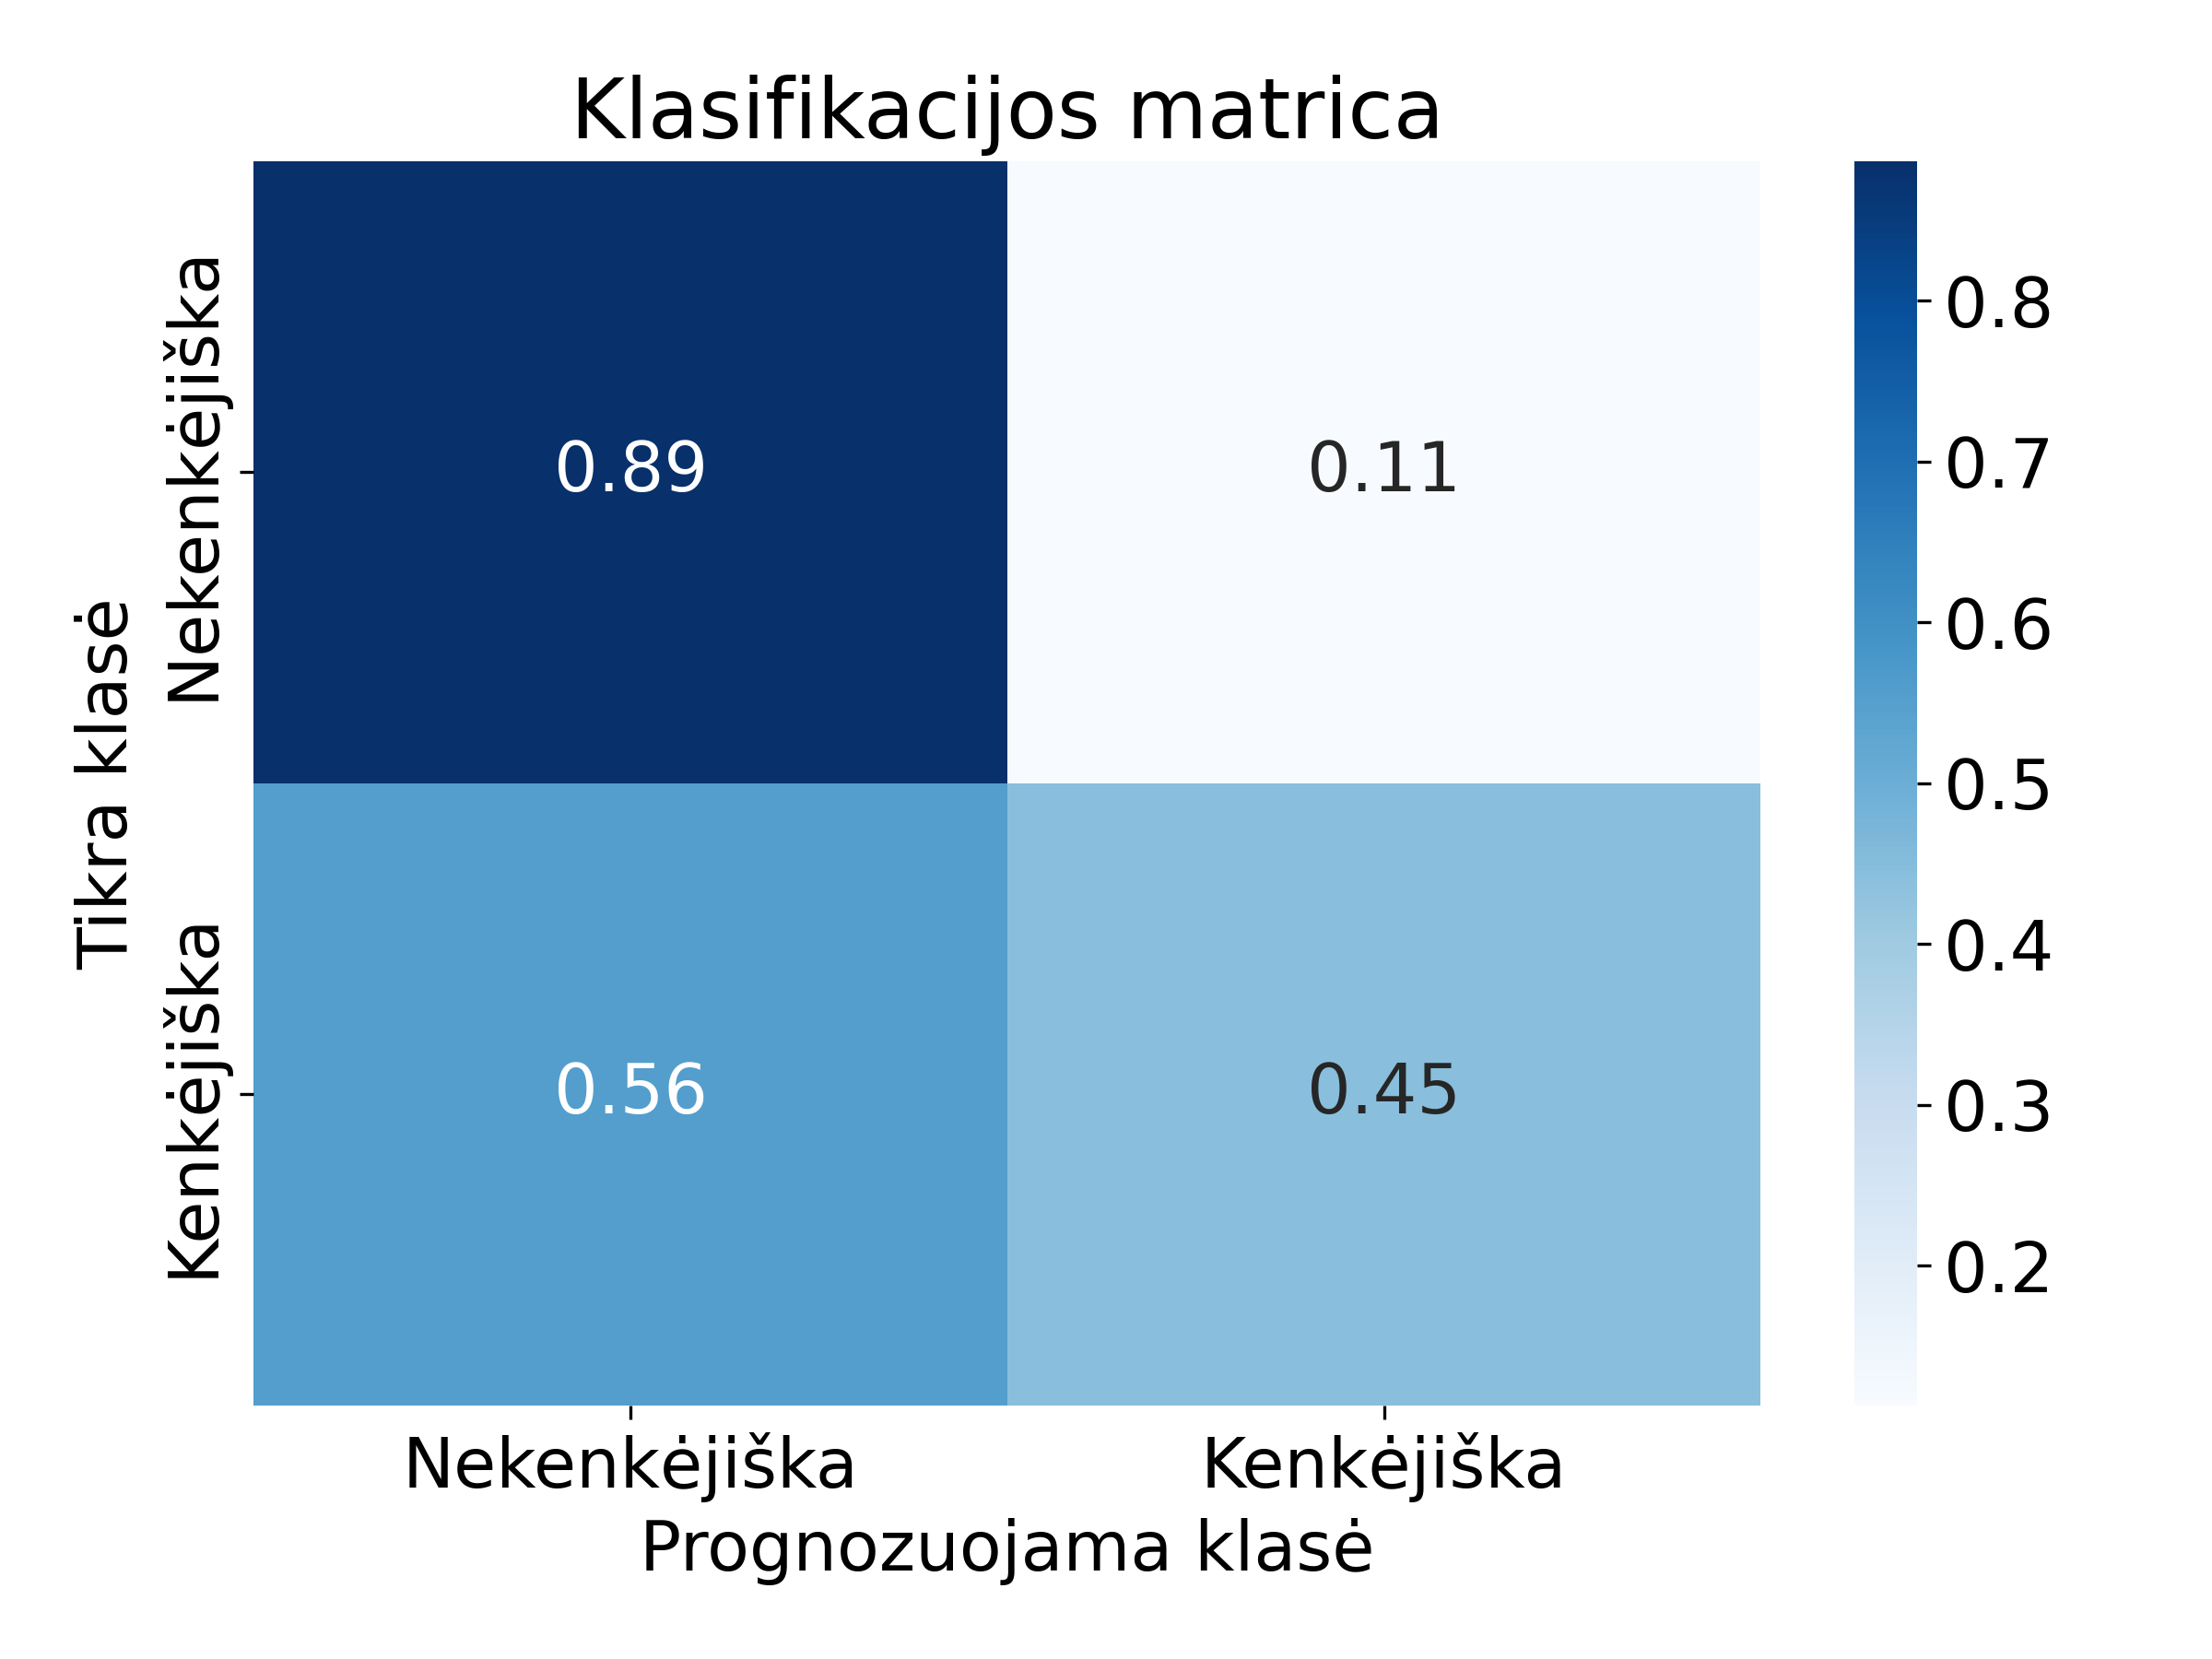
\includegraphics[width=0.5\textwidth]{images/normal_2x2.png}
    \caption{Klasifikavimo matrica}
    \label{fig:exp1:confusion}
\end{figure}

\begin{table}[h]
    \caption{Originalaus klasifikatoriaus metrikos}
    \centering
    \exptable[\accNormal]{tables/normal_2x2.csv}
    \label{tbl:exp1:metrics}
\end{table}

\footnotetext{\label{footnote:original_classifier}\textit{Originalus} klasifikatorius yra \gls{gbdt} modelis \poskyris{sec:exp:methodology}}